% Options for packages loaded elsewhere
\PassOptionsToPackage{unicode}{hyperref}
\PassOptionsToPackage{hyphens}{url}
\documentclass[
  10pt,
]{article}
\usepackage{xcolor}
\usepackage[margin=22mm]{geometry}
\usepackage{amsmath,amssymb}
\setcounter{secnumdepth}{-\maxdimen} % remove section numbering
\usepackage{iftex}
\ifPDFTeX
  \usepackage[T1]{fontenc}
  \usepackage[utf8]{inputenc}
  \usepackage{textcomp} % provide euro and other symbols
\else % if luatex or xetex
  \usepackage{unicode-math} % this also loads fontspec
  \defaultfontfeatures{Scale=MatchLowercase}
  \defaultfontfeatures[\rmfamily]{Ligatures=TeX,Scale=1}
\fi
\usepackage{lmodern}
\ifPDFTeX\else
  % xetex/luatex font selection
  \setmainfont[]{Times New Roman}
\fi
% Use upquote if available, for straight quotes in verbatim environments
\IfFileExists{upquote.sty}{\usepackage{upquote}}{}
\IfFileExists{microtype.sty}{% use microtype if available
  \usepackage[]{microtype}
  \UseMicrotypeSet[protrusion]{basicmath} % disable protrusion for tt fonts
}{}
\makeatletter
\@ifundefined{KOMAClassName}{% if non-KOMA class
  \IfFileExists{parskip.sty}{%
    \usepackage{parskip}
  }{% else
    \setlength{\parindent}{0pt}
    \setlength{\parskip}{6pt plus 2pt minus 1pt}}
}{% if KOMA class
  \KOMAoptions{parskip=half}}
\makeatother
\usepackage{longtable,booktabs,array}
\usepackage{calc} % for calculating minipage widths
% Correct order of tables after \paragraph or \subparagraph
\usepackage{etoolbox}
\makeatletter
\patchcmd\longtable{\par}{\if@noskipsec\mbox{}\fi\par}{}{}
\makeatother
% Allow footnotes in longtable head/foot
\IfFileExists{footnotehyper.sty}{\usepackage{footnotehyper}}{\usepackage{footnote}}
\makesavenoteenv{longtable}
\usepackage{graphicx}
\makeatletter
\newsavebox\pandoc@box
\newcommand*\pandocbounded[1]{% scales image to fit in text height/width
  \sbox\pandoc@box{#1}%
  \Gscale@div\@tempa{\textheight}{\dimexpr\ht\pandoc@box+\dp\pandoc@box\relax}%
  \Gscale@div\@tempb{\linewidth}{\wd\pandoc@box}%
  \ifdim\@tempb\p@<\@tempa\p@\let\@tempa\@tempb\fi% select the smaller of both
  \ifdim\@tempa\p@<\p@\scalebox{\@tempa}{\usebox\pandoc@box}%
  \else\usebox{\pandoc@box}%
  \fi%
}
% Set default figure placement to htbp
\def\fps@figure{htbp}
\makeatother
\setlength{\emergencystretch}{3em} % prevent overfull lines
\providecommand{\tightlist}{%
  \setlength{\itemsep}{0pt}\setlength{\parskip}{0pt}}
\usepackage{xeCJK}
\setCJKmainfont{Microsoft YaHei}
\setCJKmonofont{Microsoft YaHei}
\usepackage{float}
\setlength{\emergencystretch}{4em}
\setlength{\textfloatsep}{14pt plus 2pt minus 2pt}

\makeatletter
\newcommand{\fixedlabel}[2]{\phantomsection\def\@currentlabel{#2}\label{#1}}
\makeatother
\usepackage{bookmark}
\IfFileExists{xurl.sty}{\usepackage{xurl}}{} % add URL line breaks if available
\urlstyle{same}
\hypersetup{
  hidelinks,
  pdfcreator={LaTeX via pandoc}}

\author{}
\date{}

\begin{document}

\begin{center}
{\LARGE\bfseries Quantum-Inspired Search Meets Quantum Error Decoding:
Constraint-Preserving Simulated Bifurcation with Local Degeneracy
Aggregation\par}
\end{center}

\begin{center}
\small
\textbf{Jiapei Zhuang¹ and Yaocheng Chen²,*}

¹ Quantum Science Center of Guangdong-Hong Kong-Macao Greater Bay Area,
Shenzhen 518045, China

² Instituto de Astronomia, Geofísica e Ciências Atmosféricas (IAG-USP),
Universidade de São Paulo, Rua do Matão 1226, São Paulo, SP 05508-090,
Brazil

* Corresponding author:
\href{mailto:yaochengchen@usp.br}{\nolinkurl{yaochengchen@usp.br}}

\end{center}

\section{Abstract}\label{abstract}

Quantum error decoding can be formulated as Ising optimization, but
selecting the most probable error configuration does not generally
identify the logical class with the largest total probability. We
combine quantum-inspired search with local degeneracy aggregation to
estimate logical-class probabilities. Constraint-preserving simulated
bifurcation (SB) searches within each logical class in
stabilizer-generator coordinates to find a low-energy candidate. An
energy-change histogram with overlap corrections gives the exact
probability mass of the complete radius-two neighborhood around each
candidate. This local mass remains a truncated approximation to the full
logical-class mass. On rotated surface codes under code-capacity
depolarizing noise, the decoder with fixed search parameters and an
independently selected aggregation radius outperforms matching and the
tested correlated belief-propagation with ordered-statistics
post-processing baseline in all 54 held-out conditions. For distances up
to nine, its logical error rate is at most 1.1513 times the exact or
matrix-product-state reference. Exploratory increases in search effort
improve larger-distance accuracy, while aggregation improves
candidate-MAP inference at fixed candidate pools. Selected distance-13
SB and simulated-annealing configurations have similar error rates, with
SB using two to four times more flip-energy evaluations but 42--84 times
fewer sequential update rounds under the defined parallel-update model.
These results show how quantum-inspired search and local probability
aggregation can improve quantum error decoding beyond candidate
selection alone. In the tested SB--SA comparisons, this approach trades
greater total work for fewer sequential update rounds.

\section{I. Introduction}\label{i.-introduction}

Quantum error correction is a key ingredient of fault-tolerant quantum
computation, protecting logical information from physical noise through
redundant encoding and error recovery {[}\hyperlink{ref:1}{1}{]}. Recent experiments
demonstrate surface-code memories below threshold and elements of
integrated fault-tolerant architectures {[}\hyperlink{ref:2}{2},\hyperlink{ref:3}{3}{]}. The classical decoder
that interprets error syndromes also determines how well these memories
protect logical information, as decoding improvements on experimental
surface-code data illustrate {[}\hyperlink{ref:4}{4}{]}. Scaling quantum error correction
therefore requires accurate decoders with manageable computational cost.

Quantum degeneracy requires a decoder to compare classes of errors,
rather than individual errors. Errors differing by a stabilizer act
identically on encoded information; maximum-likelihood decoding
therefore selects the logical class with the largest total probability
{[}\hyperlink{ref:5}{5}{]}. In an Ising formulation, even a globally minimum-energy error
can belong to a less probable class. The challenge is to connect
low-energy search to logical-class inference.

Several approaches address different parts of this problem.
Minimum-weight perfect matching efficiently decodes suitable error
graphs {[}\hyperlink{ref:6}{6}{]}, while belief propagation with ordered-statistics
post-processing handles more general parity-check structures {[}\hyperlink{ref:7}{7}{]}.
Tensor-network methods approximate class probabilities by contraction
{[}\hyperlink{ref:8}{8},\hyperlink{ref:9}{9}{]}; Markov-chain Monte Carlo, population annealing, and worm
methods estimate probabilities or ratios through sampling
{[}\hyperlink{ref:10}{10},\hyperlink{ref:11}{11},\hyperlink{ref:12}{12}{]}. These methods address two related tasks: finding
favorable error configurations and estimating the total weight of their
logical classes.

Ising formulations connect quantum decoding to physics-inspired
optimization. Digital Annealer decoders use quadratic unconstrained
binary optimization and have been extended to circuit-level noise
{[}\hyperlink{ref:13}{13},\hyperlink{ref:14}{14}{]}. Stabilizer-generator coordinates instead satisfy syndrome
constraints exactly, as demonstrated for surface and color codes
{[}\hyperlink{ref:15}{15},\hyperlink{ref:16}{16}{]}. Iterative low-order decoding alternates between subproblems
to approximate cross-type correlations and reduce interaction order
{[}\hyperlink{ref:17}{17}{]}. These approaches establish an optimization interface, while
leaving the choice of search dynamics and the treatment of logical-class
probabilities as distinct design questions.

The quantum inspiration for simulated bifurcation (SB) comes from
dynamical approaches to optimization. Quantum annealing varies a
Hamiltonian to seek low-energy configurations {[}\hyperlink{ref:18}{18}{]}; quantum
bifurcation machines use the adiabatic evolution of Kerr-nonlinear
parametric oscillators {[}\hyperlink{ref:19}{19}{]}. SB replaces quantum-state evolution
with classical position and momentum updates derived from the
corresponding nonlinear dynamics {[}\hyperlink{ref:20}{20}{]}, an example of
physics-inspired computing on classical hardware. Synchronous SB updates
support GPU {[}\hyperlink{ref:20}{20},\hyperlink{ref:21}{21},\hyperlink{ref:22}{22}{]} and FPGA {[}\hyperlink{ref:23}{23},\hyperlink{ref:24}{24},\hyperlink{ref:25}{25}{]} implementations, with
favorable speed--quality tradeoffs on selected Ising benchmarks
{[}\hyperlink{ref:21}{21},\hyperlink{ref:22}{22}{]}. Extensions include heating and bifurcation control
{[}\hyperlink{ref:26}{26},\hyperlink{ref:27}{27}{]}, higher-order objectives {[}\hyperlink{ref:28}{28}{]}, and discrete-phase and
Potts variables {[}\hyperlink{ref:29}{29},\hyperlink{ref:30}{30}{]}. These developments extend the search
dynamics and the variables they can handle; estimating logical-class
probabilities remains a separate task.

Combining search with class-probability estimation is also an active
direction. Truncated-free-energy decoding reuses stochastic search
candidates {[}\hyperlink{ref:31}{31}{]}, while probabilistic formulations target class
partition functions {[}\hyperlink{ref:32}{32}{]}. We instead sum a complete prescribed
generator-space neighborhood around one candidate per class, including
configurations absent from the search output. At radius two, we use
locality to count these configurations with a histogram, avoiding
explicit pair enumeration.

We combine constraint-preserving SB (CP-SB) with local stabilizer-orbit
expansion (SOE) and benchmark the resulting decoder on the rotated
surface code against an exact or tensor-network reference. Building on
the established stabilizer-coordinate representation, our contributions
are as follows:

\begin{itemize}
\tightlist
\item
  \textbf{Complete local-neighborhood aggregation.}
  Constraint-preserving SB (CP-SB) supplies class-specific candidates,
  and stabilizer-orbit expansion (SOE) sums a complete prescribed
  generator-space Hamming ball around each selected center, including
  unvisited configurations.
\item
  \textbf{Exact radius-two counting.} An energy-change histogram and
  overlap corrections evaluate the local sum exactly. Counting takes
  linear work under bounded support and overlap degree once the center
  and support structure are available; this is not exact full-class
  inference.
\item
  \textbf{Controlled accuracy--resource comparisons.} Held-out testing
  and paired exploratory budget studies separate search and aggregation
  effects. At matched inference, the tested SB/SA comparisons identify
  settings with no significant accuracy difference but greater SB work
  and fewer sequential rounds. We report implementation-specific timings
  separately.
\end{itemize}

The remainder of this paper is organized as follows. Section II
constructs the decoder; Sec. III specifies evaluation and resource
measures; Sec. IV reports accuracy, aggregation effects, and costs.
Sections V and VI discuss limitations and conclude. Appendix A gives the
mathematical identities and locality conditions. Supplemental Material
contains resource, paired-effect, and extended resource views.

\section{II. METHODS: Decoder
construction}\label{ii.-methods-decoder-construction}

\hyperref[fig:1]{Figure 1} summarizes the decoding procedure. We search each
syndrome-compatible logical class for a low-weight center, sum the
probability weights over a complete neighborhood around that center, and
choose the class with the largest local mass. This sum includes
equivalent errors that the search did not visit.

Sections II A--C define the objective, feasible energy, and search;
Secs. II D--E define aggregation and its exact radius-two evaluation.
Section II F defines the matched simulated-annealing control.

\begin{figure}[H]
\centering
\pandocbounded{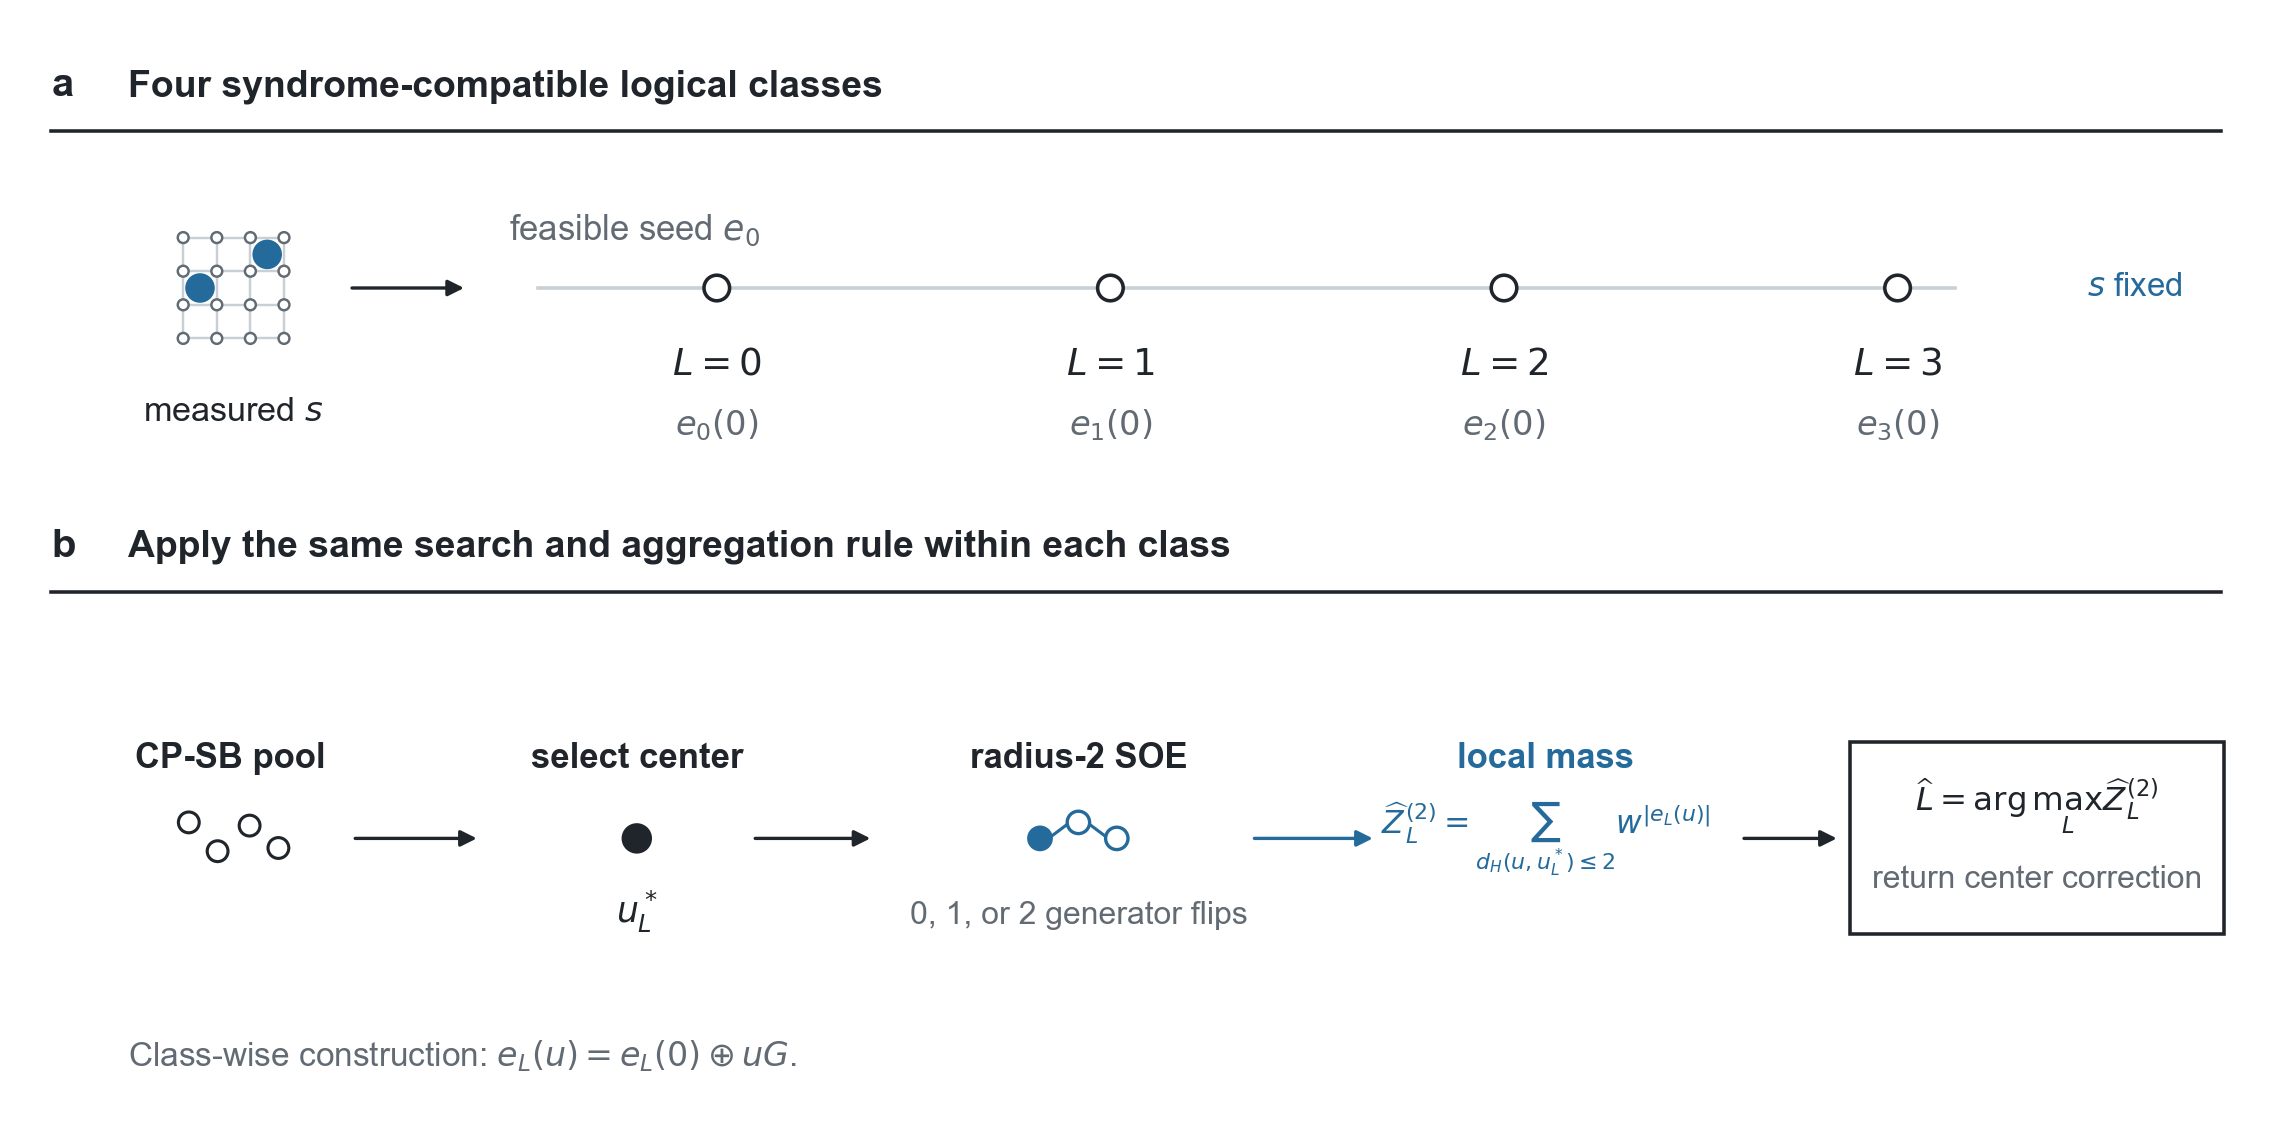
\includegraphics[width=\linewidth,height=0.62\textheight,keepaspectratio,alt={Figure 1: Constraint-preserving search and local degeneracy aggregation}]{figures/fig1_decoder_pipeline.png}}
\par\smallskip
\begin{minipage}{\linewidth}
\textbf{Figure 1. Constraint-preserving search and local degeneracy
aggregation.} (a) A measured syndrome \(s\) and a feasible seed \(e_0\)
define four syndrome-compatible logical-class seeds \(e_L(0)\),
\(L=0,1,2,3\). Stabilizer-generator flips preserve both the syndrome and
the logical class. (b) The same procedure is applied independently to
each class: constraint-preserving simulated bifurcation (CP-SB) supplies
terminal candidates, and the initial seed is also retained in the
candidate pool. The lowest Pauli-weight candidate in that pool defines
the center \(u_L^*\). Stabilizer-orbit expansion (SOE) sums
\(w^{|e_L(u)|}\), with \(w=p/[3(1-p)]\), over the complete
generator-coordinate ball \(d_H(u,u_L^*)\leq2\), giving the local mass
\(\widehat Z_L^{(2)}\). The decoder selects the class with the largest
local mass and returns its center error as the correction. The sum is
exact over this ball, not over the full logical class. The schematic
neighborhood denotes generator flips, not physical distance on the code.
\end{minipage}
\fixedlabel{fig:1}{1}
\end{figure}

\subsection{A. Decoding objective and logical
classes}\label{a.-decoding-objective-and-logical-classes}

To compare logical-class probabilities, we first need to specify the
errors in each class and their statistical weights.

We consider independent depolarizing noise on a rotated planar surface
code with distance \(d\), \(n=d^2\) data qubits, and \(m=n-1\)
independent stabilizer generators. Each qubit experiences \(X\), \(Y\),
or \(Z\) with probability \(p/3\). For a binary symplectic error vector
\(e\in\mathbb F_2^{2n}\), let \(|e|\) count its nonidentity Pauli
factors. Its probability is

\[
P(e)=(1-p)^n w^{|e|},\qquad w=\frac{p}{3(1-p)}.
\tag{1}\label{eq:1}
\]

The code encodes one logical qubit, giving four logical Pauli classes.
We use the convention \(e=(e^x,e^z)\), with \(Y\) represented by
\((1,1)\) at a qubit but contributing only one unit to \(|e|\). The
measured syndrome is denoted by \(s\).

Choose a syndrome-compatible seed \(e_0\). Let \(G\) contain the
independent stabilizer generators as rows, and let \(\ell_L\) denote
representatives of the four logical Pauli classes, \(L=0,1,2,3\). Here
\(G\in\mathbb F_2^{m\times2n}\), all products and sums in Eq. (2) are
over \(\mathbb F_2\), and the representatives \(\ell_L\) are
zero-syndrome logical operators. Every error in class \(L\) has a unique
representation

\[
e_L(u)=e_0\oplus\ell_L\oplus uG,\qquad u\in\mathbb F_2^m.
\tag{2}\label{eq:2}
\]

The unnormalized class probability is

\[
Z_L(s)=\sum_u w^{|e_L(u)|}
=\sum_u e^{-\beta E_L(u)},\quad
E_L(u)=|e_L(u)|,\quad \beta=\log\frac{3(1-p)}p.
\tag{3}\label{eq:3}
\]

The conditional class probability is \(Z_L/\sum_{L'}Z_{L'}\).
Maximum-likelihood decoding chooses the largest \(Z_L\), equivalently
the smallest effective free energy \(-\beta^{-1}\log Z_L\) in the noise
range studied. Here \(\beta\) is a statistical parameter fixed by the
noise model, not a physical device temperature.

Candidate-MAP compares the lowest energies found in each class. Without
exact search, this rule need not give minimum-weight decoding. We use
the selected candidates as centers for prescribed local mass estimates.

\subsection{B. Exact constraints and the Pauli-weight
energy}\label{b.-exact-constraints-and-the-pauli-weight-energy}

We use stabilizer coordinates to enforce the constraints and physical
Pauli weight to define the search energy.

The seed is obtained by matching the \(X\) and \(Z\) components
separately. A binary linear-system solution would also provide a
feasible seed, although its quality can affect a finite-budget search.
Equation (2) guarantees that each binary configuration preserves both
syndrome and logical class.

With generator spins \(\sigma_j=(-1)^{u_j}\), define

\[
\tau_q^x=(-1)^{(e_0\oplus\ell_L)_q^x}
\prod_{j:G_{j,q}=1}\sigma_j,
\qquad
\tau_q^z=(-1)^{(e_0\oplus\ell_L)_q^z}
\prod_{j:G_{j,n+q}=1}\sigma_j.
\]

The exact nonidentity indicator is

\[
\mathbf1[e_q\ne I]
=\frac34-\frac14\tau_q^x-\frac14\tau_q^z
-\frac14\tau_q^x\tau_q^z.
\tag{4}\label{eq:4}
\]

Summing Eq. (4) gives the Pauli-weight Hamiltonian. On this surface code
each qubit touches at most two generators of each type, so the
multilinear representation contains terms of order at most four. No
syndrome penalty or auxiliary spin is required. SB evolves continuous
variables, while their signs specify feasible physical errors. We use
\(E_L(\sigma)\) for the multilinear spin representation, which agrees
with \(E_L(u)\) at \(\sigma_j=(-1)^{u_j}\).

\subsection{C. Constraint-preserving SB candidate
search}\label{c.-constraint-preserving-sb-candidate-search}

We now use SB to search this feasible energy landscape for candidate
centers. The dynamics generates candidates for aggregation; the final
class decision also depends on their neighborhoods.

For one replica, \(x,y\in\mathbb R^m\) denote positions and momenta. We
set \(\operatorname{sgn}(0)=+1\) and recover generator bits through
\(u_j=(1-\operatorname{sgn}x_j)/2\). For each class and restart, CP-SB
evolves \(R\) replicas for \(S\) steps:

\[
y\leftarrow y+\Delta t[-(1-a_k)x+c f(\operatorname{sgn}x)],
\qquad x\leftarrow x+\Delta t\,y,
\qquad a_k=(k+1)/S.
\tag{5}\label{eq:5}
\]

The step index is \(k=0,\ldots,S-1\): the momentum update uses the
current positions, and the position update uses the newly updated
momenta. After each update, a coordinate outside \([-1,1]\) is set to
its boundary sign and its momentum is reset to zero. The initial momenta
vanish. The force is the negative gradient of the multilinear energy
evaluated at a sign vertex:

\[
f_j(\sigma)=\frac{\sigma_j}{2}
\left[E_L(\sigma^{(j)})-E_L(\sigma)\right],
\tag{6}\label{eq:6}
\]

where \(\sigma^{(j)}\) flips spin \(j\). This identity permits
evaluation from physical generator flips without introducing a quadratic
surrogate. The coupling is \(c=\kappa/\max(1,\max_j B_j)\), where
\(B_j\) is the sum of absolute coefficients of energy monomials
containing \(j\).

We combine identical monomials before evaluating this coefficient bound.

Each class receives a warm restart with initial positions
\(0.08+\mathcal N(0,0.01^2)\) and a random restart with positions
uniform in \((-0.1,0.1)\). Each restart has \(R\) replicas. Terminal
sign configurations and the initial binary seed \(u=0\) form the
candidate pool. Duplicate bitstrings are removed and the pool is sorted
by energy, with lexicographic bitstring order breaking energy ties. The
first candidate becomes the aggregation center. Intermediate trajectory
states are not added to this pool. Our budget notation \(R\times S\)
therefore corresponds to \(8R\) trajectories across four classes and two
restart modes. The fixed search configuration is \(R=8\), \(S=100\),
\(\Delta t=0.45\), and \(\kappa=0.70\).

\subsection{D. Complete local-neighborhood
aggregation}\label{d.-complete-local-neighborhood-aggregation}

Each selected center represents only one error configuration. To compare
classes, we add the probability weights of a prescribed set of
stabilizer-equivalent neighbors around that center.

The aggregation set is a complete, prescribed Hamming ball in generator
coordinates, including configurations that the search did not visit. Its
radius measures generator flips, not physical-error weight or spatial
extent. For the selected center \(u_L^*\), define

\[
\widehat Z_L^{(r)}=
\sum_{d_H(u,u_L^*)\le r} w^{E_L(u)},
\qquad \widehat L=\arg\max_L\widehat Z_L^{(r)}.
\tag{7}\label{eq:7}
\]

The decoder returns
\(e_0\oplus\ell_{\widehat L}\oplus u_{\widehat L}^*G\) as a correction.
If several computed scores agree with the maximum within relative
tolerance \(10^{-15}\) (zero absolute tolerance), the implementation
chooses the lowest class index. Independent generator rows ensure that
every term represents a distinct physical error. Thus Eq. (7) is an
exact sum over the specified ball and a lower bound on the full
unnormalized class mass. It is not an exact class probability or a
certificate for the winning class. Increasing the radius increases each
mass for fixed centers, but does not guarantee a more accurate ordering
of classes.

The radius-one and radius-two balls contain \(1+m\) and
\(1+m+\binom m2\) configurations. At \(d=13\), these counts are 169 and
14,197 per class.

\subsection{E. Exact radius-two local-mass
evaluation}\label{e.-exact-radius-two-local-mass-evaluation}

Explicit radius-two summation is costly because the number of generator
pairs grows quadratically. We compute the same local sum more
efficiently by combining additive contributions from disjoint supports
with corrections for overlapping pairs.

Let \(\Delta_j\) be the energy change from flipping generator \(j\). For
generators with disjoint physical supports,

\[
\Delta_{jk}=\Delta_j+\Delta_k.
\tag{8}\label{eq:8}
\]

We first count pair sums using a convolution of the single-flip
histogram, remove self-pairs, and divide the ordered-pair counts by two.
We then replace the additive contribution of each overlapping pair by
its true energy change. Let \(N_t\) count all radius-two configurations
with energy change \(t\), including the center, single flips, and
corrected pairs. The resulting local mass is

\[
\widehat Z_L^{(2)}=\sum_t N_t w^{E_L(u_L^*)+t}.
\]

The implementation constructs integer counts, checks their nonnegativity
and total \(1+m+\binom m2\), and sums the corresponding probabilities in
ascending Pauli-weight order. The counting identity evaluates the
prescribed local sum exactly in mathematical terms; floating-point
powers and summation introduce rounding in the implementation. The
omitted part of the logical class remains outside this sum. Appendix A
derives the full counting identity.

With bounded generator support and bounded overlap degree, the local
counting stage costs \(O(m)\) once the physical center and support
structure are available. This complexity concerns the local sum. The
archived implementation also reconstructs physical candidates with dense
matrix operations and builds a cached overlap structure; its complete
preprocessing and candidate-selection pipeline is not covered by that
linear bound.

\subsection{F. Matched simulated-annealing
control}\label{f.-matched-simulated-annealing-control}

To isolate the role of the search dynamics, we replace SB with simulated
annealing while retaining the feasible representation and aggregation
rule. This control compares the two search procedures with the same
local probability estimator.

The CP-SA control shares the feasible seeds, class Hamiltonians,
candidate-pool construction, and aggregation rule. It uses
single-generator Metropolis proposals with a geometric temperature
schedule from 2.0 to 0.05 over \(W\) sweeps, with \(C\) chains in each
restart mode. Its budget is denoted \(C\times W\). Warm chains start at
\(u=0\), while random chains start from independent uniform binary
states. Each sweep visits a fresh random permutation of all \(m\)
generators in each chain. Non-increasing proposals are accepted; an
increase \(\Delta E>0\) is accepted with probability
\(e^{-\Delta E/T}\). For \(W\ge2\), the geometric schedule includes both
endpoints; a single sweep uses the initial temperature. This search
temperature is distinct from the channel parameter \(\beta\) in Eq. (3).
Although the SA solver also records best-ever states, the benchmark
prediction pool uses only terminal states and the seed, with the same
deduplication and tie rules as SB. A sweep contains \(m\) sequential
proposals per chain and is not equivalent in work to one SB step.
Holding the inference radius fixed allows the two search procedures to
be compared without changing the probability estimator.

\section{III. Evaluation design}\label{iii.-evaluation-design}

We evaluate the fixed-configuration decoder, examine how search and
aggregation affect its accuracy, and measure their computational costs.
We first test held-out errors after independent radius selection, then
explore budgets and inference rules. Resource counts and implementation
timings are reported separately.

\subsection{A. Evaluation stages and data
separation}\label{a.-evaluation-stages-and-data-separation}

\hyperref[tab:1]{Table 1} separates configuration selection, held-out testing, and
exploratory studies so that the role of each dataset is explicit. A shot
is one physical Pauli error; shared shots produce paired outcomes. LER
is failure probability per code-capacity shot, not per measurement
round.

\par
\noindent\begin{minipage}{\linewidth}
\fixedlabel{tab:1}{1}\textbf{Table 1. Evaluation stages.}

\begin{longtable}[]{@{}
  >{\raggedright\arraybackslash}p{(\linewidth - 4\tabcolsep) * \real{0.3333}}
  >{\raggedright\arraybackslash}p{(\linewidth - 4\tabcolsep) * \real{0.3333}}
  >{\raggedright\arraybackslash}p{(\linewidth - 4\tabcolsep) * \real{0.3333}}@{}}
\toprule\noalign{}
\begin{minipage}[b]{\linewidth}\raggedright
Stage
\end{minipage} & \begin{minipage}[b]{\linewidth}\raggedright
Conditions and samples
\end{minipage} & \begin{minipage}[b]{\linewidth}\raggedright
Role
\end{minipage} \\
\midrule\noalign{}
\endhead
\bottomrule\noalign{}
\endlastfoot
Selection & \(d=5,\allowbreak 7,\allowbreak 9\),\allowbreak  \(p=0.10,\allowbreak 0.12\); respectively 3,\allowbreak 000,\allowbreak  2,\allowbreak 000,\allowbreak  and
1,\allowbreak 000 shots per cell; 12,\allowbreak 000 total & Select SOE radius with the search
parameters fixed \\
Main evaluation grid & Six distances \(3,\allowbreak 5,\allowbreak 7,\allowbreak 9,\allowbreak 11,\allowbreak 13\),\allowbreak  nine noise rates
\(0.04,\allowbreak 0.05,\allowbreak 0.06,\allowbreak 0.08,\allowbreak 0.10,\allowbreak 0.12,\allowbreak 0.14,\allowbreak 0.16,\allowbreak 0.18\); 7.12 million shots &
Held-out evaluation of CP-SB \(8\times100\),\allowbreak  radius two \\
Budget scan & First 10,\allowbreak 000 shots per cell at \(d=9,\allowbreak 11,\allowbreak 13\),\allowbreak 
\(p=0.08\)--0.18; incomplete configuration coverage at 0.18 &
Exploratory allocation of replicas/chains and steps/sweeps \\
Extended-budget evaluation & CP-SB \(8\times400\) at \(d=11,\allowbreak 13\); full
cells for \(p\ge0.08\),\allowbreak  first 100,\allowbreak 000 shots for \(p\le0.06\) & Evaluate
a rule chosen after examining the budget scan \\
\end{longtable}
\end{minipage}
\par

Before the held-out grid was generated, radius two was selected only if
it reduced pooled selection-set failures and passed an exact paired test
at 0.05. It corrected 70 shots missed by radius one and missed 40
corrected by radius one, giving \(P_{\rm test}=0.0054\). The resulting
main decoder is CP-SB \(8\times100\) with SOE radius two. Selection and
held-out noise seeds are disjoint. Grid cell sizes range from 10,000 to
one million shots.

The budget scan includes SB configurations \(8\times100\),
\(16\times100\), \(32\times100\), \(64\times100\), \(8\times200\),
\(8\times400\), and \(32\times400\), and SA configurations
\(8\times25\), \(8\times50\), \(8\times100\), \(8\times200\),
\(16\times100\), and \(32\times200\). Each is evaluated with
candidate-MAP and SOE radii one and two where available. Five
configurations were run at \(p=0.18\). We used these data to choose the
extended-budget rule, so its evaluation provides exploratory evidence
rather than an independent held-out confirmation.

\subsection{B. Baselines and reference
validation}\label{b.-baselines-and-reference-validation}

We use matching and correlated BP+OSD as accuracy baselines, CP-SA to
isolate search dynamics at fixed representation and inference, and REF
as a reference for logical-class decisions.

The matching baseline decodes the two Pauli components separately.
Unit-weight matching and the tested probability-weighted PyMatching
implementation produce identical grid predictions. The main BP baseline
is correlated BP+OSD-CS with order seven, min-sum updates, and \(3n\)
iterations. Here \(H_X\) and \(H_Z\) are the binary X- and Z-stabilizer
support matrices; \(H_Z\) detects the X component and \(H_X\) detects
the Z component. Its binary check matrix is

\[
\begin{pmatrix}H_Z&0&H_Z\\0&H_X&H_X\end{pmatrix},
\tag{9}\label{eq:9}
\]

with \(X,Z,Y\) component priors \(p/3\). The three binary blocks
\((x,z,y)\) map to physical components \(e^x=x\oplus y\) and
\(e^z=z\oplus y\). The implementation checks syndrome compatibility but
imposes no explicit per-qubit exclusivity constraint on the three binary
events. Our comparison concerns this specific correlated baseline,
rather than BP-based decoders in general. It improves on the separately
decoded BP+OSD baseline in all grid cells.

REF is exact class enumeration at \(d=3\). For \(d=5,7,9\), it uses an
MPS decoder with bond dimension \(\chi=32\). At \(d=11,13\), it uses
\(\chi=16\), with \(\chi=32\) replacements on selected difficult shots,
capped at 3,000 per cell. Difficult shots were identified by a tested
decoder failing or disagreeing with the \(\chi=16\) prediction. When the
difficult set exceeds the cap, 3,000 shots are selected by sampling
without replacement with a fixed random state. Because this targeted
check uses simulation information, it validates the reference rather
than defining a deployable decoder-selection rule.

On the checked difficult subsets at \(d\ge11\), the \(\chi=16/32\)
comparison has at most two disagreements per cell, and the
\(\chi=32/64\) comparison has at most one. The latter check covers 18
cells with 401--3,000 shots each. These observations support a stable
numerical reference on the tested subsets; they do not certify exact ML
for every larger-code shot. Ratios below one on a finite sample need not
imply a decoder with lower expected error than exact ML.

\subsection{C. Statistical
comparisons}\label{c.-statistical-comparisons}

We distinguish uncertainty in individual LERs from uncertainty in their
differences. Paired outcomes on shared shots allow us to assess the
latter.

LER intervals are Wilson 95\% intervals. Paired differences use exact
two-sided McNemar tests with Holm correction within each comparison
family. Supplemental Fig. S2 instead shows conservative Clopper--Pearson
difference intervals with Bonferroni allocation; these have at least
95\% coverage under the binomial shot model but are not simultaneous
Holm-adjusted intervals. Filled markers report the corrected tests,
whereas interval crossings reflect the separate interval construction.
We use pooled discordant counts across cells only descriptively.

Holm families contain all 54 main-grid cells for each fixed decoder
pair, including the different REF implementations. Budget families are
specific to a configuration pair and inference rule over available
cells: the three radius-two families in Supplemental Fig. S2 contain 15,
18, and 18 cells. Extended-budget families contain 18 cells per decoder
pair. Missing configurations are not imputed; correction does not cover
all exploratory choices.

Each discordant-event probability receives a Clopper--Pearson interval
with failure probability 0.025. Subtracting opposite endpoints gives an
interval for LER(A) minus LER(B); negative values favor A.

\subsection{D. Computational resources and
timing}\label{d.-computational-resources-and-timing}

To assess computational cost alongside accuracy, we distinguish total
search work, sequential depth, and measured CPU time. We define the
first two resources as

\[
N_{\Delta E}^{\rm SB}=8RSm,\quad
N_{\Delta E}^{\rm SA}=8CWm;\qquad
D_{\rm SB}=S,\quad D_{\rm SA}=Wm.
\tag{10}\label{eq:10}
\]

The first counts single-generator flip-energy evaluations. The second
counts update rounds when logical classes, restarts, and replicas or
chains run in parallel, while SA updates within a chain remain
sequential. These quantities exclude setup, inference, communication,
and the internal cost of an energy evaluation. They are neither
end-to-end operation counts nor measured hardware latency. Alternative
parallel SA implementations are outside this comparison.

CPU times are medians over 100 unique nontrivial syndromes at p=0.10 on
an AMD EPYC 9754 node, using single-process Python 3.11/NumPy 2.4. SB
batches updates, SA performs Python proposals, and matching/BP+OSD use
compiled components. Thread counts default to one only when environment
variables are unset. Because the archive does not record the actual
values, we cannot independently verify single-thread execution.

\hyperref[fig:4]{Figure 4} uses optimized sparse-search/histogram-SOE end-to-end timings
and archived baseline timings, linked to existing accuracy records at
the same noise probability. Fixed χ=16 MPS accuracy is taken from its
own grid record, not from the adaptive REF identity. \hyperref[tab:2]{Table 2} also
retains a historical explicit-SOE stage for comparison. Both campaigns
use 100 unique nontrivial syndromes per condition at p=0.10; the later
campaign reuses syndromes and solver seeds. Optimized times exclude
once-per-code support preparation. Search-only excludes seeding and
aggregation; end-to-end CP includes both. Raw-log ``total'' may combine
inference evaluations and is not a stage definition. MPS timings use
fixed bond dimension, not the targeted-validation REF pipeline.

\section{IV. Results}\label{iv.-results}

We first report held-out accuracy, then examine budget allocation,
aggregation at fixed candidates, and computational costs. Figures 2--5
give the main comparisons; Supplemental Figs. S1--S2 retain resource
comparisons and paired-effect views.

\subsection{A. Accuracy of the fixed-configuration
decoder}\label{a.-accuracy-of-the-fixed-configuration-decoder}

We begin with the configuration fixed before the held-out evaluation.
The baselines measure its practical gains, while REF identifies the
remaining accuracy gap. The main decoder improves on matching and
correlated BP+OSD in all 54 held-out cells, each significant after Holm
correction (largest adjusted p values: 8.7×10⁻¹² and 0.0077). Pooled
discordant wins/losses are 55,081/17,007 against matching and
41,739/21,099 against correlated BP+OSD.

For distances up to nine, LER is at most 1.1513 times REF; 27 of these
36 cells show no significant paired difference under Sec. III C's Holm
families, which does not establish equivalence. Maximum ratios rise to
approximately 1.33 and 1.87 at distances 11 and 13, revealing a
larger-code gap with fixed parameters.

\begin{figure}[H]
\centering
\pandocbounded{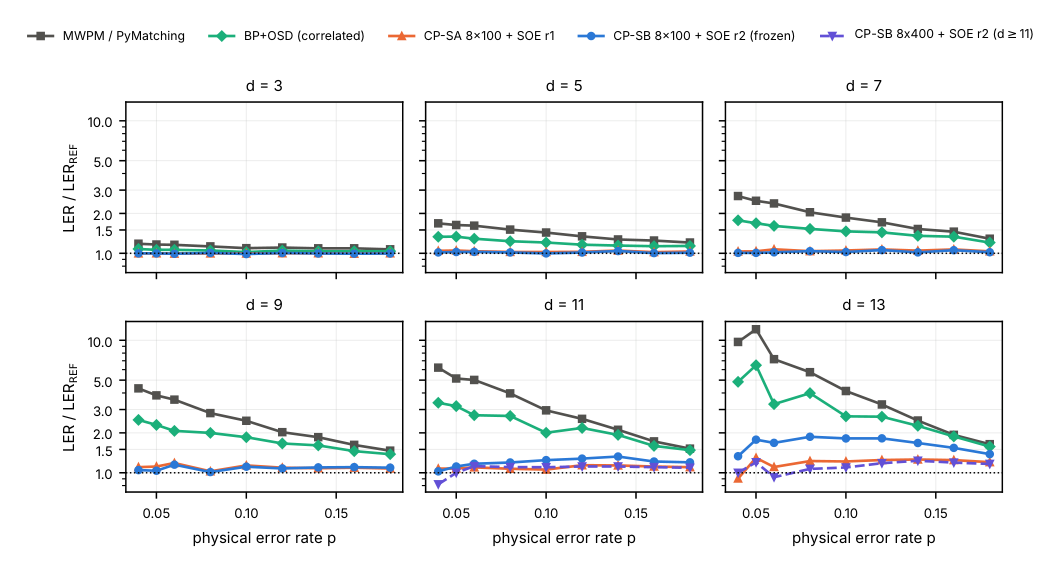
\includegraphics[width=\linewidth,height=0.62\textheight,keepaspectratio,alt={Figure 2}]{figures/preview_fig2.png}}
\par\smallskip
\begin{minipage}{\linewidth}
\textbf{Figure 2. Accuracy relative to REF.} Each panel shows one code
distance, with physical error probability on the horizontal axis and
LER/REF on the vertical axis. The horizontal reference corresponds to a
ratio of one. Solid main-method curves use the fixed-configuration
decoder. Purple downward-triangle extended-budget curves at distances 11
and 13 are exploratory and use their own evaluated subsets, including
only 100,000 shots per low-noise cell. Ratios are point estimates; no
paired ratio intervals are implied. The reference has few failures at
low noise and large code distances, so these ratios are especially
sensitive to sampling. The CP-SA curve uses radius one, whereas the main
CP-SB curve uses radius two; their separation does not isolate the
search dynamics.
\end{minipage}
\fixedlabel{fig:2}{2}
\end{figure}

\subsection{B. Finite-size behavior and search-budget
allocation}\label{b.-finite-size-behavior-and-search-budget-allocation}

The gap at larger code distances raises two questions: whether more
search improves accuracy and how to allocate that search effort.
Increasing the SB step count from 100 to 400 lowers point-estimated LER
in all 18 extended-budget cells at distances 11 and 13, with 12
significant after Holm correction. For p≥0.08, REF ratios change from
1.20--1.33 to 1.09--1.12 at distance 11 and from 1.38--1.87 to
1.07--1.23 at distance 13. These improvements provide exploratory
evidence for the selected budget rule, rather than independent
confirmation.

CP-SB 8×400 and 32×100 use equal flip-energy evaluation counts
(4,300,800 at distance 13), not necessarily equal runtime or end-to-end
work. At distance 13 and p=0.12, radius-two REF ratios on the
10,000-shot subset are approximately 1.17 and 1.28. The longer run
wins/loses 1,935/1,643 discordant shots across 15 cells, with lower LER
in nine but only one significant difference after Holm correction. This
does not establish a universal allocation advantage.

The distance-11/13 crossing moves from approximately p=0.1167 to 0.1581,
versus 0.1765 for REF. Estimates linearly interpolate log-LER
differences across p intervals 0.10--0.12, 0.14--0.16, and 0.16--0.18,
respectively, without crossing confidence intervals. They demonstrate
budget sensitivity, not an asymptotic threshold: sizes are limited and
the larger budget was selected after inspecting the scan.

\begin{figure}[H]
\centering
\pandocbounded{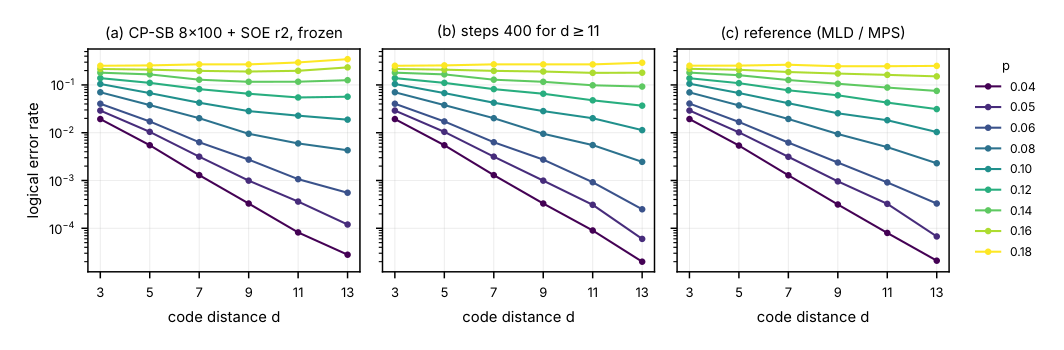
\includegraphics[width=\linewidth,height=0.62\textheight,keepaspectratio,alt={Figure 3}]{figures/preview_fig3.png}}
\par\smallskip
\begin{minipage}{\linewidth}
\textbf{Figure 3. Finite-size behavior under fixed and enlarged search
budgets.} Physical error probability labels the curves; the horizontal
axis is code distance and the vertical axis is logical error rate.
Panels compare the fixed-configuration decoder, the decoder with 400
steps at distances 11 and 13, and REF. The change of curve ordering
illustrates finite-budget sensitivity, rather than an established
asymptotic threshold. The reported crossing is where the distance-11 and
distance-13 LERs become equal as functions of physical error
probability; it is not a crossing between the colored curves in this
distance-axis view.
\end{minipage}
\fixedlabel{fig:3}{3}
\end{figure}

\begin{figure}[H]
\centering
\pandocbounded{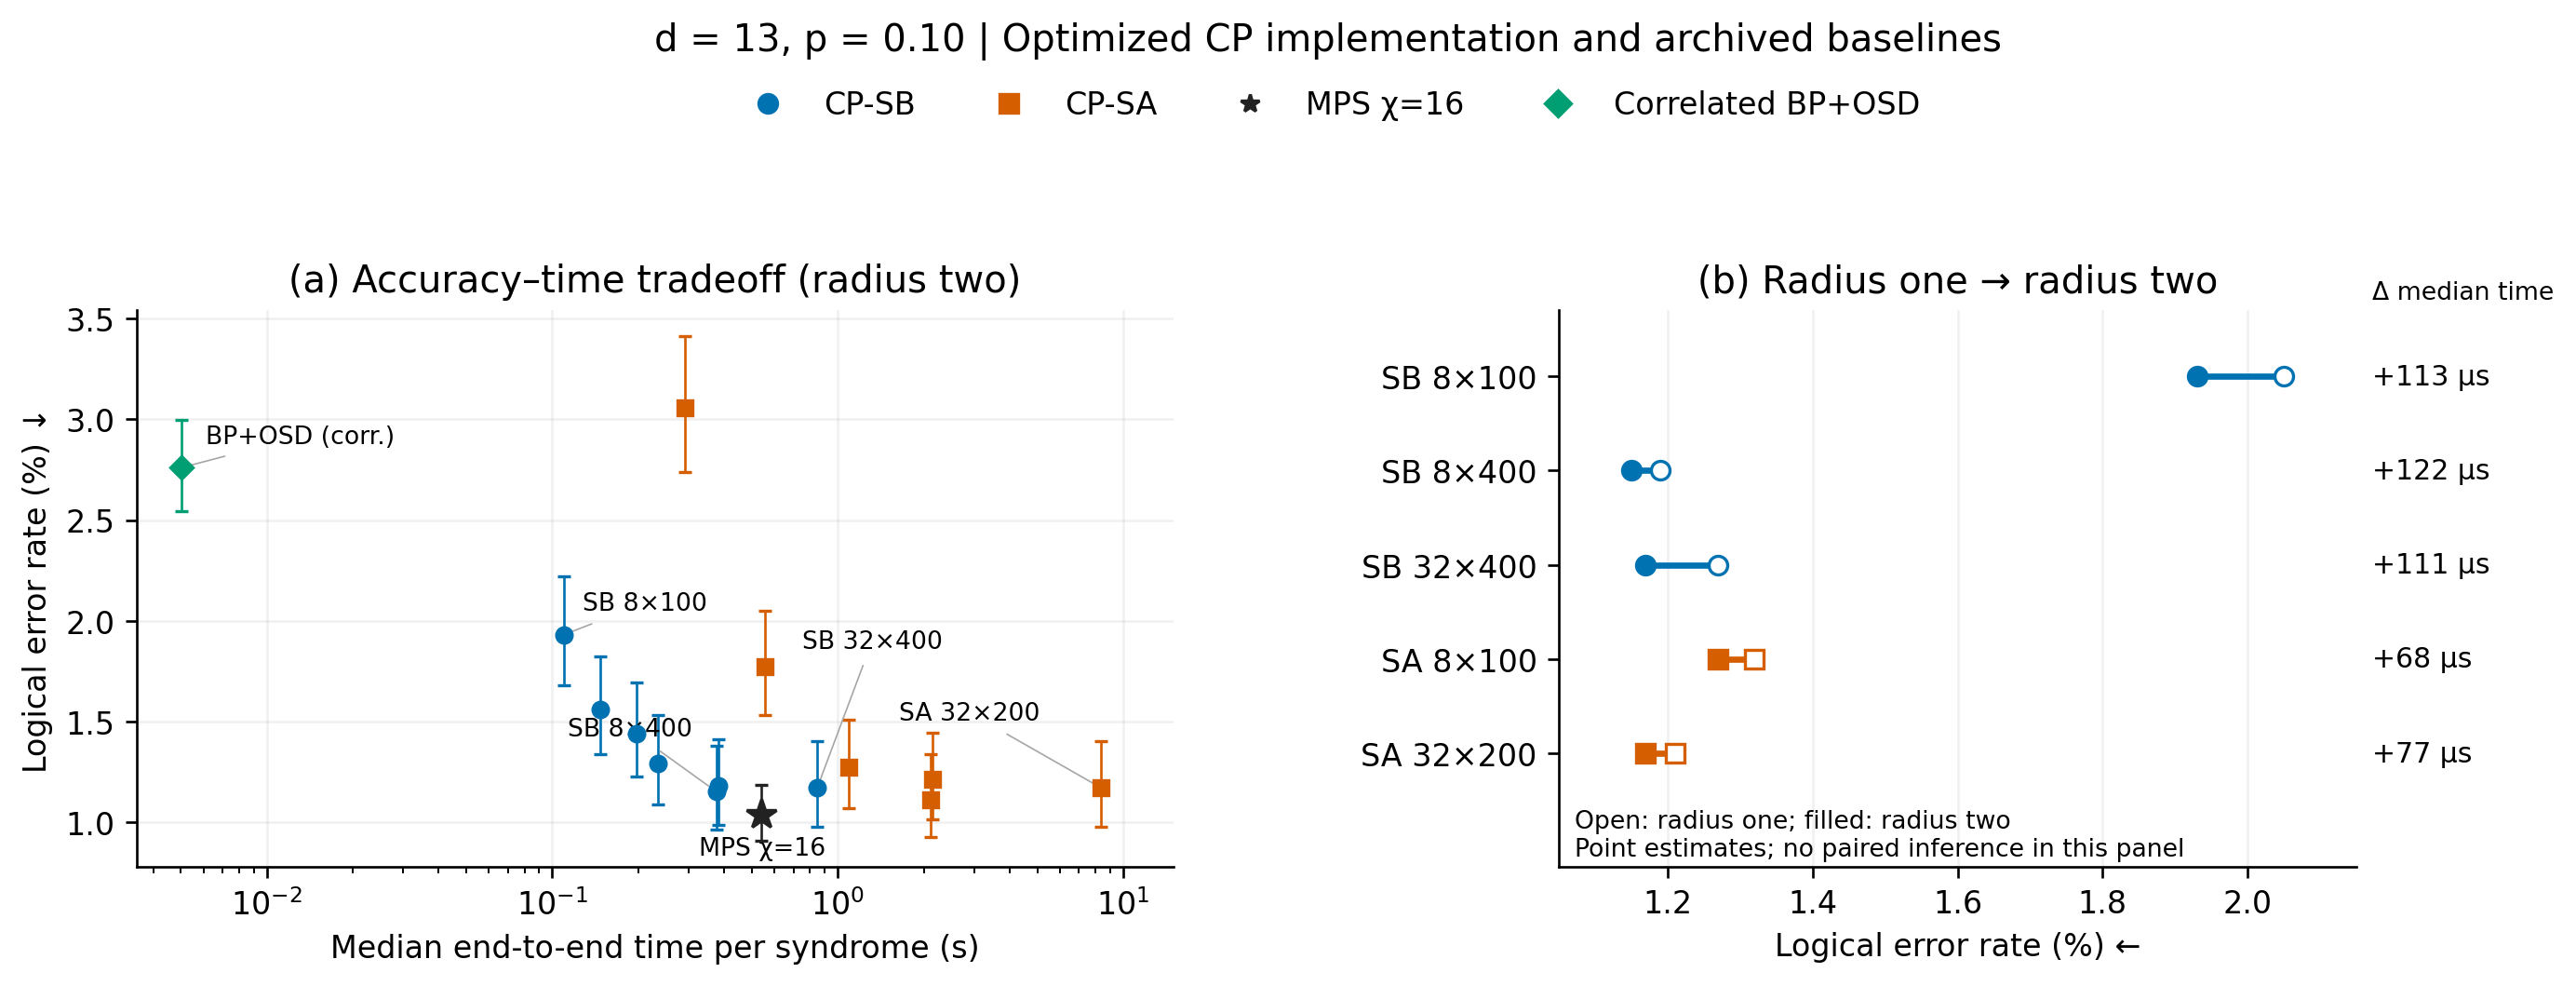
\includegraphics[width=\linewidth,height=0.62\textheight,keepaspectratio,alt={Figure 4}]{figures/figure4_optimized.png}}
\par\smallskip
\begin{minipage}{\linewidth}
\textbf{Figure 4. Accuracy and end-to-end time at distance 13 and
p=0.10.} (a) All archived SB and SA budgets with radius-two aggregation,
compared with fixed-bond-dimension MPS (χ=16) and correlated BP+OSD.
Vertical bars are pointwise Wilson 95\% intervals: 10,000 accuracy shots
per CP configuration and 20,000 per baseline. The logarithmic time axis
shows medians over 100 unique nontrivial syndromes. CP times include
seeding, search, and aggregation but exclude once-per-code preparation.
We use optimized CP timings and archived baseline timings, combined with
existing accuracy observations; no accuracy experiments were rerun here.
(b) Selected configurations: open and filled markers show radius-one and
radius-two LER point estimates. Labels give the difference between their
end-to-end time medians, not the median of per-syndrome time
differences. This panel supplies no paired significance test or timing
confidence interval. SB labels denote replicas × steps; SA labels denote
chains × sweeps.
\end{minipage}
\fixedlabel{fig:4}{4}
\end{figure}

\hyperref[fig:4]{Figure 4} shows an implementation-specific accuracy--time tradeoff. SB
8×400 takes 0.375 s versus 0.540 s for fixed χ=16 MPS, about 30.5\% less
time, with LER point estimates of 1.15\% and 1.035\%, respectively. This
does not establish accuracy equivalence or dominance over MPS. For the
five selected configurations, radius-two aggregation lowers the LER
point estimate with differences of approximately 68--122 μs between
end-to-end medians; these small timing differences lack uncertainty
estimates. Algorithmic resource and paired budget comparisons remain in
Supplemental Figs. S1--S2.

\subsection{C. What local aggregation adds after
search}\label{c.-what-local-aggregation-adds-after-search}

Changing the search budget changes the candidates. We now hold the
candidate pools fixed to isolate the effect of the inference rule. At
fixed candidate pools, replacing candidate-MAP with local aggregation
improves accuracy without assuming global search optimality. On the
distance-13, p=0.12, 10,000-shot subset, CP-SB 32×400 gives REF ratios
1.382, 1.115, and 1.096 for MAP, radius one, and radius two; CP-SA
32×200 gives 1.376, 1.099, and 1.093. These examples use larger budgets
than \hyperref[fig:5]{Fig. 5}'s fixed and 8×400 searches.

Radius two further lowers LER in 50 of 54 grid cells, with three
significant after correction and pooled wins/losses of 5,222/4,337. The
radius was selected before this grid was generated, so these comparisons
describe its subsequent performance.

\begin{figure}[H]
\centering
\pandocbounded{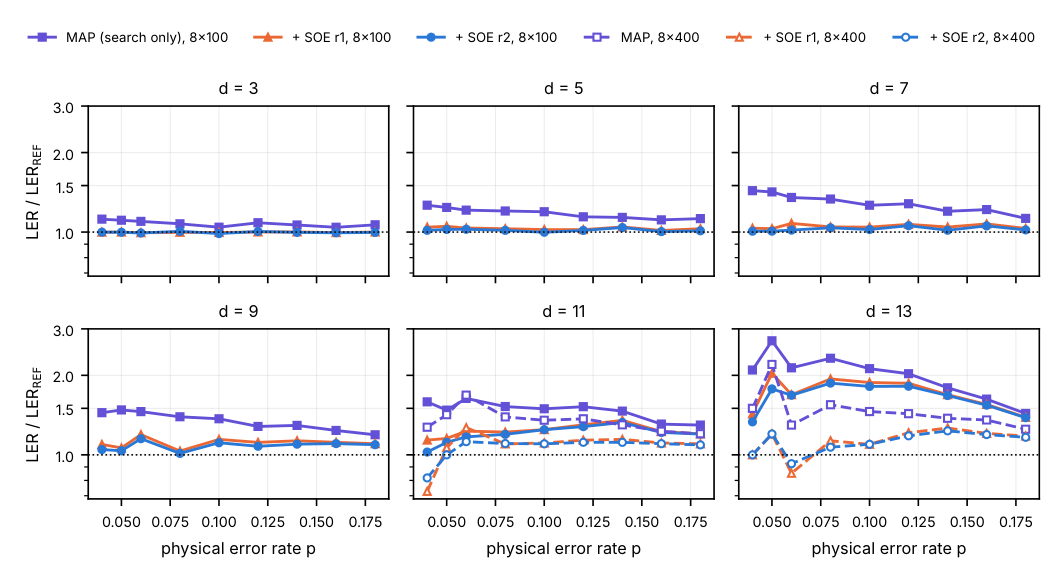
\includegraphics[width=\linewidth,height=0.62\textheight,keepaspectratio,alt={Figure 5}]{figures/preview_fig5.png}}
\par\smallskip
\begin{minipage}{\linewidth}
\textbf{Figure 5. Candidate-MAP and local aggregation.} The six-panel
figure compares candidate-MAP, SOE radius one, and SOE radius two
against REF as a function of physical error probability. Solid curves
use the fixed-budget search, and dashed open-marker curves use the
extended budget where available. Comparisons at fixed search isolate a
change of inference rule. Vertical gaps are changes in decoding
performance, not an additive causal decomposition of error sources. In
particular, the residual radius-two gap cannot be assigned entirely to
truncation without independently controlling search quality.
\end{minipage}
\fixedlabel{fig:5}{5}
\end{figure}

At the largest scanned SB and SA budgets, radius-two REF ratios remain
approximately 1.075--1.129 at distance 13 and p≥0.10. No cell in
Supplemental Fig. S2's right panel passes Holm correction. The similar
residual gaps motivate further work on the estimator. They establish
neither equivalent decisions nor search convergence, and stronger search
could still help.

\subsection{D. Work, sequential rounds, and elapsed
time}\label{d.-work-sequential-rounds-and-elapsed-time}

We now compare the resources required for these accuracy levels,
treating algorithmic counts separately from implementation-specific
elapsed time. At distance 13, SB 8×400 uses four times the evaluations
of SA 8×100 but 400 rather than 16,800 rounds; SB 32×400 uses twice the
evaluations of SA 32×200 but 400 rather than 33,600 rounds. Neither
radius-two comparison has a significant difference in its 18-cell Holm
family (Supplemental Figs. S1--S2). The work--depth tradeoff is
therefore two to four times more evaluations for 42--84 times fewer
rounds, not a uniformly superior searcher.

\par
\noindent\begin{minipage}{\linewidth}
\fixedlabel{tab:2}{2}\textbf{Table 2. Selected archived CPU timings at distance 13.} Medians
in seconds per unique nontrivial syndrome, measured at \(p=0.10\). Rows
identify the timed stage; search-only values are not end-to-end decoder
times. CP search and end-to-end rows use the optimized
sparse-search/histogram implementation. The explicit-SOE row remeasures
the historical algorithm in the optimized timing campaign; both SOE rows
specify SB 8×100. Baseline rows retain their archived implementations,
and the execution-environment limits in Sec. III D apply.

\begin{longtable}[]{@{}lr@{}}
\toprule\noalign{}
Configuration or stage & Time (s) \\
\midrule\noalign{}
\endhead
\bottomrule\noalign{}
\endlastfoot
PyMatching decoder & 0.000043 \\
Correlated BP+OSD decoder & 0.0050 \\
MPS, \(\chi=16\) & 0.540 \\
MPS, \(\chi=32\) & 3.269 \\
SB search, \(8\times100\) & 0.104 \\
SB search, \(8\times400\) & 0.369 \\
SB search, \(32\times400\) & 0.841 \\
SA search, \(8\times100\) & 1.084 \\
SA search, \(32\times200\) & 8.33 \\
Explicit radius-two SOE, SB 8×100 (historical) & 3.540 \\
Histogram radius-two SOE, SB 8×100 (optimized) & 0.000816 \\
End to end: SB \(8\times100\) + radius two & 0.110 \\
End to end: SB \(8\times400\) + radius two & 0.375 \\
\end{longtable}
\end{minipage}
\par

The stage timings show how much fast local counting reduces the cost of
aggregation. For distance-13 SB 8×100 pools, histogram aggregation
reduces radius-two evaluation from 3.53979 s to 0.00081604 s within the
optimized timing campaign, approximately 4,300-fold; this is a
stage-specific, not decoder-wide, speedup. For CP-SB 8×100, CP-SB 8×400
at distances at least 11, and CP-SA 8×100, checks of radii one and two
over the same 42,800 decodes found identical candidate pools between
sparse and full-vector search, unchanged decisions including ties, and
maximum relative class-score differences of 1.2×10⁻¹⁵. These finite
checks do not cover every budget in \hyperref[fig:4]{Fig. 4}, guarantee bit-identical
scores, or supply new accuracy data.

The fixed-χ comparison in \hyperref[fig:4]{Fig. 4} does not measure the complete
targeted-validation REF runtime. SB/SA CPU ratios also mix batching and
language overhead with algorithmic structure. Hardware latency requires
measuring memory traffic, synchronization, and occupancy; fewer update
rounds alone do not establish acceleration.

\section{V. Discussion}\label{v.-discussion}

The method uses exact aggregation over a complete prescribed local
neighborhood to turn low-energy candidates into estimates of
logical-class mass. Different logical classes can have different
fractions of omitted mass. Exact local evaluation therefore does not
certify the ordering of the full class masses. Held-out tests and
fixed-candidate comparisons support this search-and-aggregation
approach, although an accuracy gap to REF remains at larger code
distances.

Both search and mass estimation may contribute to that gap. The
matched-work comparisons suggest examining run length alongside replica
count, but do not establish a universally preferred allocation. Similar
residual errors under the largest tested SB and SA budgets do not
establish convergence or isolate truncation as the cause. Future
comparisons can separate these effects by varying search at fixed
inference and the estimator at fixed candidate pools. Extensions using
multiple centers or adaptive neighborhoods must avoid duplicate counting
and account for their computational overhead.

Histogram counting makes aggregation inexpensive in the tested
implementation, subject to the support and overlap conditions of Sec. II
E. This reduction in aggregation time is separate from the work--depth
tradeoff of the SB search. Neither historical CPU timings nor the
optimized comparison establishes dominance over the adaptive REF
pipeline. Demonstrating hardware benefit requires matched
implementations and measurements of end-to-end latency, throughput,
memory traffic, and synchronization.

Extending the method beyond the surface code requires both a suitable
coordinate representation and the locality needed for efficient
counting. The coordinate construction extends algebraically to binary
stabilizer codes with an independent generator basis and \(4^k\) logical
Pauli classes for \(k\) encoded qubits. Small fixed-\(k\) families with
suitable local bases, including planar color codes, are natural tests;
stabilizer-coordinate optimization already exists for color codes
{[}\hyperlink{ref:16}{16}{]}. Efficient radius-two counting additionally requires bounded
supports and overlap, and the surface-code four-body representation is
not general. Local mass depends on the basis; dependent generators can
duplicate physical errors. For high-rate qLDPC codes, logical-class
enumeration is a further obstacle. This is not yet an efficient general
qLDPC decoder.

Circuit-level noise requires us to work with fault mechanisms rather
than data-qubit errors. In principle, kernel coordinates of stacked
detector and logical-observable maps preserve both records, but
constructing a useful basis does not itself establish efficient local
counting. Such an extension would need to account for fault likelihoods,
possible global basis elements, mechanism incidence, and nonuniform
weights. Circuit-level decoding accuracy and runtime have not been
evaluated here.

\section{VI. Conclusion}\label{vi.-conclusion}

We have combined simulated-bifurcation search with probability
aggregation over complete prescribed stabilizer-coordinate neighborhoods
for logical-class inference. The coordinates preserve syndrome and
logical class without penalty terms, while a support-based histogram
evaluates the radius-two mass exactly without enumerating all generator
pairs. The resulting local mass remains an approximation to the full
logical-class mass. On held-out rotated-surface-code data under
independent depolarizing noise, the main decoder improves over the
tested matching and correlated BP+OSD baselines, while exploratory
increases in the SB step count improve larger-distance accuracy. At
fixed candidate pools, local aggregation improves on candidate-MAP
inference. In the selected SB--SA comparisons, SB uses more flip-energy
evaluations but fewer sequential update rounds; the corresponding
hardware latency remains to be measured. These results support a
search-then-aggregate approach to code-capacity decoding. Further
progress depends on designing search budgets, local mass estimators, and
their implementation together.

\section{Appendix A. Exact identities and locality
conditions}\label{appendix-a.-exact-identities-and-locality-conditions}

This appendix derives the identities underlying the feasible
coordinates, flip-energy force, and radius-two histogram in Sec. II, and
states the locality assumptions required for efficient evaluation.

\subsection{A.1. Constraint preservation and
counting}\label{a.1.-constraint-preservation-and-counting}

All binary operations are over \(\mathbb F_2\), and Pauli errors are
identified up to overall phase. Let \(H\) be the syndrome map in the
\((X\mid Z)\) convention, including the symplectic pairing, so that
\(HG^T=0\). When the measured checks are the rows of \(G\) in the same
order, \(H=GJ\), where

\[
J=\begin{pmatrix}0&I_n\\I_n&0\end{pmatrix}.
\]

Reordering the measured checks permutes the rows of this map
accordingly. Logical representatives have zero syndrome, so Eq. (2)
gives

\[
He_L(u)^T=He_0^T+H\ell_L^T+HG^Tu^T=s.
\]

Varying \(u\) multiplies the error by a stabilizer and therefore
preserves its logical class. Since
\(\operatorname{rank}_{\mathbb F_2}G=m\), equality \(uG=vG\) implies
\(u=v\). A generator-space ball thus maps injectively to physical Pauli
errors up to phase. Dependent generators would preserve the constraints
but could count a physical error more than once.

For \(0<p<1\), the weight \(w=p/[3(1-p)]\) is positive and finite. For
any nonnegative integer radius \(r\), the ball \(\mathcal B_r(u_L^*)\)
contains its center, and

\[
Z_L-\widehat Z_L^{(r)}
=\sum_{u\notin\mathcal B_r(u_L^*)}w^{E_L(u)}\ge0,
\qquad 0<\widehat Z_L^{(r)}\le Z_L.
\]

This subset-sum bound applies to unnormalized masses. It does not bound
the fraction omitted from each class, certify the class ordering, or
provide calibrated conditional probabilities.

\subsection{A.2. Flip energies and
force}\label{a.2.-flip-energies-and-force}

We next derive the interaction force used by SB from discrete flip
energies.

Any multilinear energy can be written as
\(E(\sigma)=A_j(\sigma_{\ne j})+\sigma_j b_j(\sigma_{\ne j})\), where
neither \(A_j\) nor \(b_j\) depends on \(\sigma_j\). Flipping spin \(j\)
gives

\[
\Delta_j=E(\sigma^{(j)})-E(\sigma)=-2\sigma_j b_j.
\]

Since \(\sigma_j^2=1\) at a spin vertex,

\[
\frac{\sigma_j}{2}\Delta_j=-b_j
=-\frac{\partial E}{\partial\sigma_j},
\]

which proves Eq. (6). The function \(b_j\) here is distinct from the
coefficient bound \(B_j\) used to normalize the coupling in Sec. II C.
The SB update evaluates this identity at
\(\sigma=\operatorname{sgn}(x)\), with the stated zero-sign convention;
it does not identify the interaction force with \(-\nabla E(x)\) at
arbitrary continuous positions. The identity holds for the chosen
energy; it proves neither monotonic energy decrease nor convergence of
the SB updates.

\subsection{A.3. Radius-two
histogram}\label{a.3.-radius-two-histogram}

We now derive a counting identity for the complete radius-two sum that
avoids explicit pair enumeration.

Fix a logical class and its center \(u_L^*\), and write
\(E_0=E_L(u_L^*)\). Let \(\epsilon_j\) be the binary unit vector in
generator coordinate \(j\). All changes are measured from the same
center:

\[
\Delta_j=E_L(u_L^*\oplus\epsilon_j)-E_0,
\qquad
\Delta_{jk}=E_L(u_L^*\oplus\epsilon_j\oplus\epsilon_k)-E_0
\quad(j<k).
\]

Write \(h_t=\#\{j:\Delta_j=t\}\) for integer \(t\), and define
\((h*h)_t=\sum_{a\in\mathbb Z}h_a h_{t-a}\). This convolution counts
ordered generator pairs, including self-pairs. Removing the self-pairs
and dividing by two gives the histogram of additive changes over all
unordered distinct pairs:

\[
P_t=\frac12\left[(h*h)_t-\sum_j\mathbf1[t=2\Delta_j]\right].
\tag{A1}\label{eq:A1}
\]

Because the Pauli-weight objective is a sum of single-qubit indicators,
generators with disjoint physical-qubit supports satisfy
\(\Delta_{jk}=\Delta_j+\Delta_k\). Let \(\mathcal O\) contain each pair
\(j<k\) whose physical-qubit supports intersect, including overlap
between X and Z components on the same qubit. For each overlapping pair,
we replace the additive contribution with the contribution from its true
energy change. Including the center and all single flips, the exact
radius-two histogram is

\[
N_t=\mathbf1[t=0]+h_t+P_t
+\sum_{(j,k)\in\mathcal O}
\bigl(\mathbf1[t=\Delta_{jk}]-\mathbf1[t=\Delta_j+\Delta_k]\bigr).
\tag{A2}\label{eq:A2}
\]

Thus \(N_t\ge0\) and \(\sum_tN_t=1+m+\binom m2\): each overlap
correction preserves the total count. With independent generator rows,
these counts enumerate distinct physical errors, and

\[
\widehat Z_L^{(2)}=\sum_tN_t w^{E_0+t}.
\]

The histogram identities are exact in integer arithmetic; the
implementation uses fixed-width integer counts and floating-point
probability evaluation. Exact counting requires the integer counts to
stay within range; the numerical scores remain subject to floating-point
rounding and range limits. Exact evaluation of this local sum does not
extend to the omitted part of the logical class.

If every generator touches at most a fixed \(K\) qubits, single-flip
changes lie in \([-K,K]\) and pair changes in \([-2K,2K]\). If
\(|\mathcal O|=O(m)\), the single-flip counts and overlap corrections
require \(O(m)\) local work, with fixed-size convolution. Bounded
overlap degree is sufficient for this condition. This bound assumes that
the physical center and support incidence data are already available. It
does not cover the complete candidate-selection or decoding pipeline.
Dense construction of the overlap matrix, dense reconstruction of
candidates, pool scoring, and cache storage are separate costs in the
archived code. Even cached-structure lookup constructs a key from the
dense generator matrix. The bound also relies on the integer
Pauli-weight objective: arbitrary position-dependent likelihood weights
require a fresh complexity analysis, and correlated objectives require
rechecking disjoint-support additivity.

\section{References}\label{references}

\begin{enumerate}
\def\labelenumi{[\arabic{enumi}]}
\tightlist
\item
  \hypertarget{ref:1}{} B. M. Terhal, \href{https://doi.org/10.1103/RevModPhys.87.307}{Quantum
  error correction for quantum memories}, Rev.~Mod. Phys. \textbf{87},
  307 (2015).
\item
  \hypertarget{ref:2}{} Google Quantum AI and Collaborators,
  \href{https://doi.org/10.1038/s41586-024-08449-y}{Quantum error
  correction below the surface code threshold}, Nature \textbf{638}, 920
  (2025).
\item
  \hypertarget{ref:3}{} D. Bluvstein \emph{et al.},
  \href{https://doi.org/10.1038/s41586-025-09848-5}{A fault-tolerant
  neutral-atom architecture for universal quantum computation}, Nature
  \textbf{649}, 39 (2026).
\item
  \hypertarget{ref:4}{} J. Bausch \emph{et al.},
  \href{https://doi.org/10.1038/s41586-024-08148-8}{Learning
  high-accuracy error decoding for quantum processors}, Nature
  \textbf{635}, 834 (2024).
\item
  \hypertarget{ref:5}{} E. Dennis, A. Kitaev, A. Landahl, and J. Preskill,
  \href{https://doi.org/10.1063/1.1499754}{Topological quantum memory},
  J. Math. Phys. \textbf{43}, 4452 (2002).
\item
  \hypertarget{ref:6}{} O. Higgott, \href{https://doi.org/10.1145/3505637}{PyMatching: A
  Python package for decoding quantum codes with minimum-weight perfect
  matching}, ACM Trans. Quantum Comput. \textbf{3}, 16 (2022).
\item
  \hypertarget{ref:7}{} J. Roffe, D. R. White, S. Burton, and E. Campbell,
  \href{https://doi.org/10.1103/PhysRevResearch.2.043423}{Decoding
  across the quantum low-density parity-check code landscape}, Phys.
  Rev.~Research \textbf{2}, 043423 (2020).
\item
  \hypertarget{ref:8}{} S. Bravyi, M. Suchara, and A. Vargo,
  \href{https://doi.org/10.1103/PhysRevA.90.032326}{Efficient algorithms
  for maximum likelihood decoding in the surface code}, Phys. Rev.~A
  \textbf{90}, 032326 (2014).
\item
  \hypertarget{ref:9}{} C. T. Chubb, \href{https://arxiv.org/abs/2101.04125}{General tensor
  network decoding of 2D Pauli codes}, arXiv:2101.04125 (2021).
\item
  \hypertarget{ref:10}{} A. Hutter, J. R. Wootton, and D. Loss,
  \href{https://doi.org/10.1103/PhysRevA.89.022326}{Efficient Markov
  chain Monte Carlo algorithm for the surface code}, Phys. Rev.~A
  \textbf{89}, 022326 (2014).
\item
  \hypertarget{ref:11}{} F. Martínez-García, F. R. F. Pereira, and P. Parrado-Rodríguez,
  \href{https://doi.org/10.3390/e28010091}{Near-optimal decoding
  algorithm for color codes using population annealing}, Entropy
  \textbf{28}, 91 (2026).
\item
  \hypertarget{ref:12}{} Z. Tobias, N. P. Breuckmann, and B. Placke,
  \href{https://arxiv.org/abs/2603.05428}{Optimal Decoding with the
  Worm}, arXiv:2603.05428 (2026).
\item
  \hypertarget{ref:13}{} J. Fujisaki, H. Oshima, S. Sato, and K. Fujii,
  \href{https://doi.org/10.1103/PhysRevResearch.4.043086}{Practical and
  scalable decoder for topological quantum error correction with an
  Ising machine}, Phys. Rev.~Research \textbf{4}, 043086 (2022).
\item
  \hypertarget{ref:14}{} J. Fujisaki, K. Maruyama, H. Oshima, S. Sato, T. Sakashita, Y.
  Takeuchi, and K. Fujii,
  \href{https://doi.org/10.1103/PhysRevResearch.5.043261}{Quantum error
  correction with an Ising machine under circuit-level noise}, Phys.
  Rev.~Research \textbf{5}, 043261 (2023).
\item
  \hypertarget{ref:15}{} Y. Takeuchi, Y. Takada, T. Sakashita, J. Fujisaki, H. Oshima, S. Sato,
  and K. Fujii, \href{https://arxiv.org/abs/2311.07973}{Comparative
  study of decoding the surface code using simulated annealing under
  depolarizing noise}, arXiv:2311.07973 (2023).
\item
  \hypertarget{ref:16}{} Y. Takada, Y. Takeuchi, and K. Fujii,
  \href{https://doi.org/10.1103/PhysRevResearch.6.013092}{Ising model
  formulation for highly accurate topological color codes decoding},
  Phys. Rev.~Research \textbf{6}, 013092 (2024).
\item
  \hypertarget{ref:17}{} Y. Liu, W. Zeng, P. Li, Y. Liu, G. Huang, Y. Liu, D. Wang, J. Wu, and
  L. Lao, \href{https://arxiv.org/abs/2606.12301}{An iterative Ising
  decoder for quantum error correction codes}, arXiv:2606.12301 (2026).
\item
  \hypertarget{ref:18}{} T. Kadowaki and H. Nishimori,
  \href{https://doi.org/10.1103/PhysRevE.58.5355}{Quantum annealing in
  the transverse Ising model}, Phys. Rev.~E \textbf{58}, 5355 (1998).
\item
  \hypertarget{ref:19}{} H. Goto, \href{https://doi.org/10.1038/srep21686}{Bifurcation-based
  adiabatic quantum computation with a nonlinear oscillator network},
  Sci. Rep.~\textbf{6}, 21686 (2016).
\item
  \hypertarget{ref:20}{} H. Goto, K. Tatsumura, and A. R. Dixon,
  \href{https://doi.org/10.1126/sciadv.aav2372}{Combinatorial
  optimization by simulating adiabatic bifurcations in nonlinear
  Hamiltonian systems}, Sci. Adv. \textbf{5}, eaav2372 (2019).
\item
  \hypertarget{ref:21}{} H. Goto, K. Endo, M. Suzuki, Y. Sakai, T. Kanao, Y. Hamakawa, R.
  Hidaka, M. Yamasaki, and K. Tatsumura,
  \href{https://doi.org/10.1126/sciadv.abe7953}{High-performance
  combinatorial optimization based on classical mechanics}, Sci. Adv.
  \textbf{7}, eabe7953 (2021).
\item
  \hypertarget{ref:22}{} J. Pawłowski, P. Tarasiuk, J. Tuziemski, Ł. Pawela, and B. Gardas,
  \href{https://doi.org/10.1103/qcws-8kgm}{Toward quantum scaling
  advantage in approximate optimization}, Phys. Rev.~Applied
  \textbf{26}, 014024 (2026).
\item
  \hypertarget{ref:23}{} T. Kashimata, M. Yamasaki, R. Hidaka, and K. Tatsumura,
  \href{https://doi.org/10.1109/ACCESS.2024.3374089}{Efficient and
  scalable architecture for multiple-chip implementation of simulated
  bifurcation machines}, IEEE Access \textbf{12}, 36606 (2024).
\item
  \hypertarget{ref:24}{} F. Orlando, D. Volpe, G. Orlandi, M. Graziano, F. Riente, and M.
  Vacca, \href{https://arxiv.org/abs/2510.12407}{High-Parallel
  FPGA-Based Discrete Simulated Bifurcation for Large-Scale
  Optimization}, arXiv:2510.12407 (2025).
\item
  \hypertarget{ref:25}{} B. Yao, D. Ebler, X. Shi, J. Wang, F. Zhang, W. Zhang, and J. Sun,
  \href{https://doi.org/10.1038/s41467-026-75119-0}{Precision meets
  speed through an FPGA-based natively sparse Ising machine for
  combinatorial optimization}, Nat. Commun. \textbf{17}, 8549 (2026).
\item
  \hypertarget{ref:26}{} T. Kanao and H. Goto,
  \href{https://doi.org/10.1038/s42005-022-00929-9}{Simulated
  bifurcation assisted by thermal fluctuation}, Commun. Phys.
  \textbf{5}, 153 (2022).
\item
  \hypertarget{ref:27}{} H. Goto, R. Hidaka, and K. Tatsumura,
  \href{https://doi.org/10.1103/2qd9-x6v8}{Edge-of-chaos-enhanced
  quantum-inspired algorithm for combinatorial optimization}, Phys.
  Rev.~Applied \textbf{25}, 044011 (2026).
\item
  \hypertarget{ref:28}{} T. Kanao and H. Goto,
  \href{https://doi.org/10.35848/1882-0786/acaba9}{Simulated bifurcation
  for higher-order cost functions}, Appl. Phys. Express \textbf{16},
  014501 (2023).
\item
  \hypertarget{ref:29}{} Y. Chen and J. Zhuang,
  \href{https://github.com/yaochengchen/clock-dsb}{Clock-variable
  discrete simulated bifurcation: A GPU algorithm for large-scale
  discrete-phase optimization}, unpublished manuscript (2026).
\item
  \hypertarget{ref:30}{} J. Zhuang and Y. Chen,
  \href{https://github.com/yaochengchen/PdSB}{Beyond one-hot encoding:
  Native Potts discrete simulated bifurcation breaks G-set Max-k-Cut
  records}, unpublished manuscript (2026).
\item
  \hypertarget{ref:31}{} Y. Liu, W. Zeng, J. Wu, and L. Lao,
  \href{https://arxiv.org/abs/2609.03928}{Approximate maximum-likelihood
  decoding via truncated free energies}, arXiv:2609.03928 (2026).
\item
  \hypertarget{ref:32}{} R. Krishnamoorthy \emph{et al.},
  \href{https://arxiv.org/abs/2608.25545}{Certified decoding of quantum
  LDPC codes}, arXiv:2608.25545 (2026).
\end{enumerate}

\end{document}
